%%%%%%%%%%%%%%%%%%%%%%%%%%%%%%%%%%%%%%%%%%%%%%%%%%
\section{Il rilevatore ALICE e i suoi componenti}
A seguire verrà fatta un'introduzione sulle caratteristiche di un rilevatore in generale e quali sono le grandezze principali, e in seguito sulle principali caratteristiche e componenti del rivelatore ALICE.

\subsection{Caratterizzazione di un rilevatore e le grandezze principali}
Lo scopo di un rilevatore è quello di determinare le caratteristiche della particella, come la sua identità (i.e. la sua massa), l'impulso, il suo vertice di origine, l'energia e altre caratteristiche.
Per semplificare il processo di misura si definiscono delle grandezze associabili alle particelle.
Consideriamo un generico rilevatore di forma cilindrica con al suo centro il punto di interazione (IP) e con l'asse rivolto lungo l'asse $z$.
Considerando ora una particella che viene emessa dall'IP (magari dopo uno scattering) con quadrimpulso iniziale (in \textit{}{natural units}) $p^\nu = (E,\vec p)$, con $\vec p = (p_{x}, p_{y}, p_{z})$.
Questa prosegue il suo cammino finché non interagisce con il rilevatore.
L'\emph{impulso trasverso} $p_t$ della particella è definito come 
\begin{equation}
    p_t^2 = p_x^2 + p_y^2
\end{equation}
e la sua \emph{rapidità} come 
\begin{equation}
    y = \dfrac12 \ln\left(\dfrac{E+p_z}{E-p_z}\right)
\end{equation}
Le utilità di queste grandezze è che il primo è invariante per boost lungo l'asse $z$, visto che coinvolge solamente le componenti trasversali, mentre la seconda è una misura di quanto una particella sia direzionata verso l'asse $z$.
Infatti se la particella viene emessa in una direzione giacente nel piano $xy$, si ha che $p_z=0$ perciò $y=0$.
Se invece la direzione è coincidente con l'asse $z$ si ha che $E = \pm p_z$ (supponendo un regime ultra-relativistico per cui $|\vec p| \gg m$) e quindi $y\to \pm\infty$.
Applicando un boost lungo l'asse $z$ la rapidità si trasforma seguendo la seguente espressione ($y\to y'$)
\begin{equation}
    y' = y + \dfrac12\sqrt{\dfrac{1-\beta}{1+\beta}}
\end{equation}
quindi la rapidità varia di una costante legata al boost effettuato.
Un altro vantaggio nell'utilizzare questo parametro è che la differenza di rapidità tra due particelle nel loro sistema di riferimento è uguale a quella nel sistema di riferimento del laboratorio, ossia che $y_1-y_2 = y_1'-y_2'$.

Tuttavia negli esperimenti non sempre viene utilizzato questo parametro, perché richiede la conoscenza sia di $E$ che di $p_z$.
Quindi si procede a definire la \emph{pseudorapidità}, definita come 
\begin{equation}
    \eta = -\ln\tan\dfrac\theta2
\end{equation}
con $\theta$ l'angolo di scattering, ossia l'angolo tra l'asse del cilindro e la direzione di $\vec p$.
Negli esperimenti di LHC viene usata questa variabile al posto della rapidità perché con $p\gg m$ (e quindi $E\approx p$) si ha che $y\approx \eta$, il che ne spiega l'utilizzo.
In \autoref{fig:cms} si mostra una rappresentazione schematica del sistema di coordinate utilizzato convenzionalmente nei rilevatori di LHC.

\begin{figure}[htb]
    \centering
    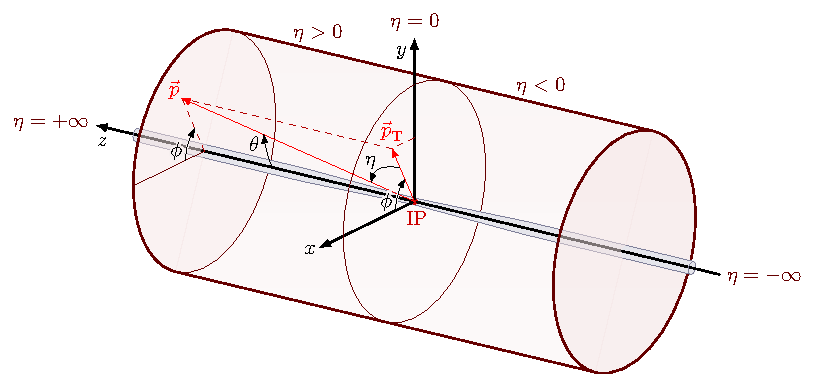
\includegraphics[width=0.9\textwidth]{image/1-alice/axis3D_CMS.pdf}
    \caption{Rappresentazione schematica del sistema di coordinate di un rilevatore in generale di LHC. "IP" è il punto di interazione, $\phi$ è l'angolo assiale, $\theta$ è l'angolo di scattering, $\eta$ è la pseudorapidità. Le particelle provengono da $-\infty$ dell'asse $z$. (Autore: \href{https://tikz.net/axis3d_cms/}{Izaak Neutelings})}
    \label{fig:cms}
\end{figure}

\subsection{Caratteristiche e principali componenti di ALICE}
Il rilevatore ALICE, ossia il complesso dei rilevatori dell'esperimento ALICE, è situato nel Punto di Interazione 2 (IP2) di LHC.
Esso è costituito da una massa di 10,000 tonnellate, lungo 26 m, alto e largo 16 m.
Occupandosi di ioni pesanti, esso deve assicurarsi di gestire bene le problematicità legate alle alte densità di particelle cariche (al tempo di design erano previste 8000 particelle cariche per unità di pseudo-rapidità, a rapidità centrali $|\eta|<1$).
Per questo motivo, per assicurarsi di ottenere delle misure di alta qualità, è necessario l'utilizzo di sensori con elevata granularità e risoluzione spaziale. 
Inoltre esso deve garantire di poter di misurare particelle che, avendo massa maggiore, verranno prodotte con l'impulso trasverso $p_t$ minore, e allo stesso modo poter effettuare la misura di particelle con $p_t$ maggiore.
Quindi, affinché ALICE possa misurare queste particelle, è necessario che il rivelatore possa ricostruire particelle in un intervallo di $p_t$ ampio, nello specifico da 100 MeV/$c$ a 100 GeV/$c$.

La struttura di ALICE è molto complessa, ma si possono individuare due parti principali:
\begin{itemize}
    \item una sezione centrale ("\emph{central barrel}") dove sono collocati i rilevatori più importanti, la maggior parte disposti geometricamente in una configurazione a guscio cilindrico.
    Questi sensori sono racchiusi da un magnete solenoidale (\emph{L3 Magnet}) che genera un campo magnetico uniforme, in direzione del suo asse, con un'intensità di $0.5$ T, necessario per la misura dell'impulso per le particelle cariche.
    In questa sezione si svolgono le mansioni più importanti di ALICE, ossia l'IDentificazione delle Particelle (PID), il tracciamento della traiettoria e la determinazione di processi che avvengono a una pseudo-rapidità di $|\eta| < 1$;
    \item una sezione esterna al magnete solenoidale per la rilevazione di muoni e comunque per misure a una pseudo-rapidità di $-4<\eta<-2.5$.
    In questa zona è presente anche un altro magnete detto \emph{magnete dipolare} con il compito di filtrare particelle indesiderate e permettere la misura dell'impulso dei muoni.
\end{itemize}
Una raffigurazione con le principali componenti di ALICE è riportata in \autoref{fig:alice}.

\begin{figure}[htb]
    \centering
    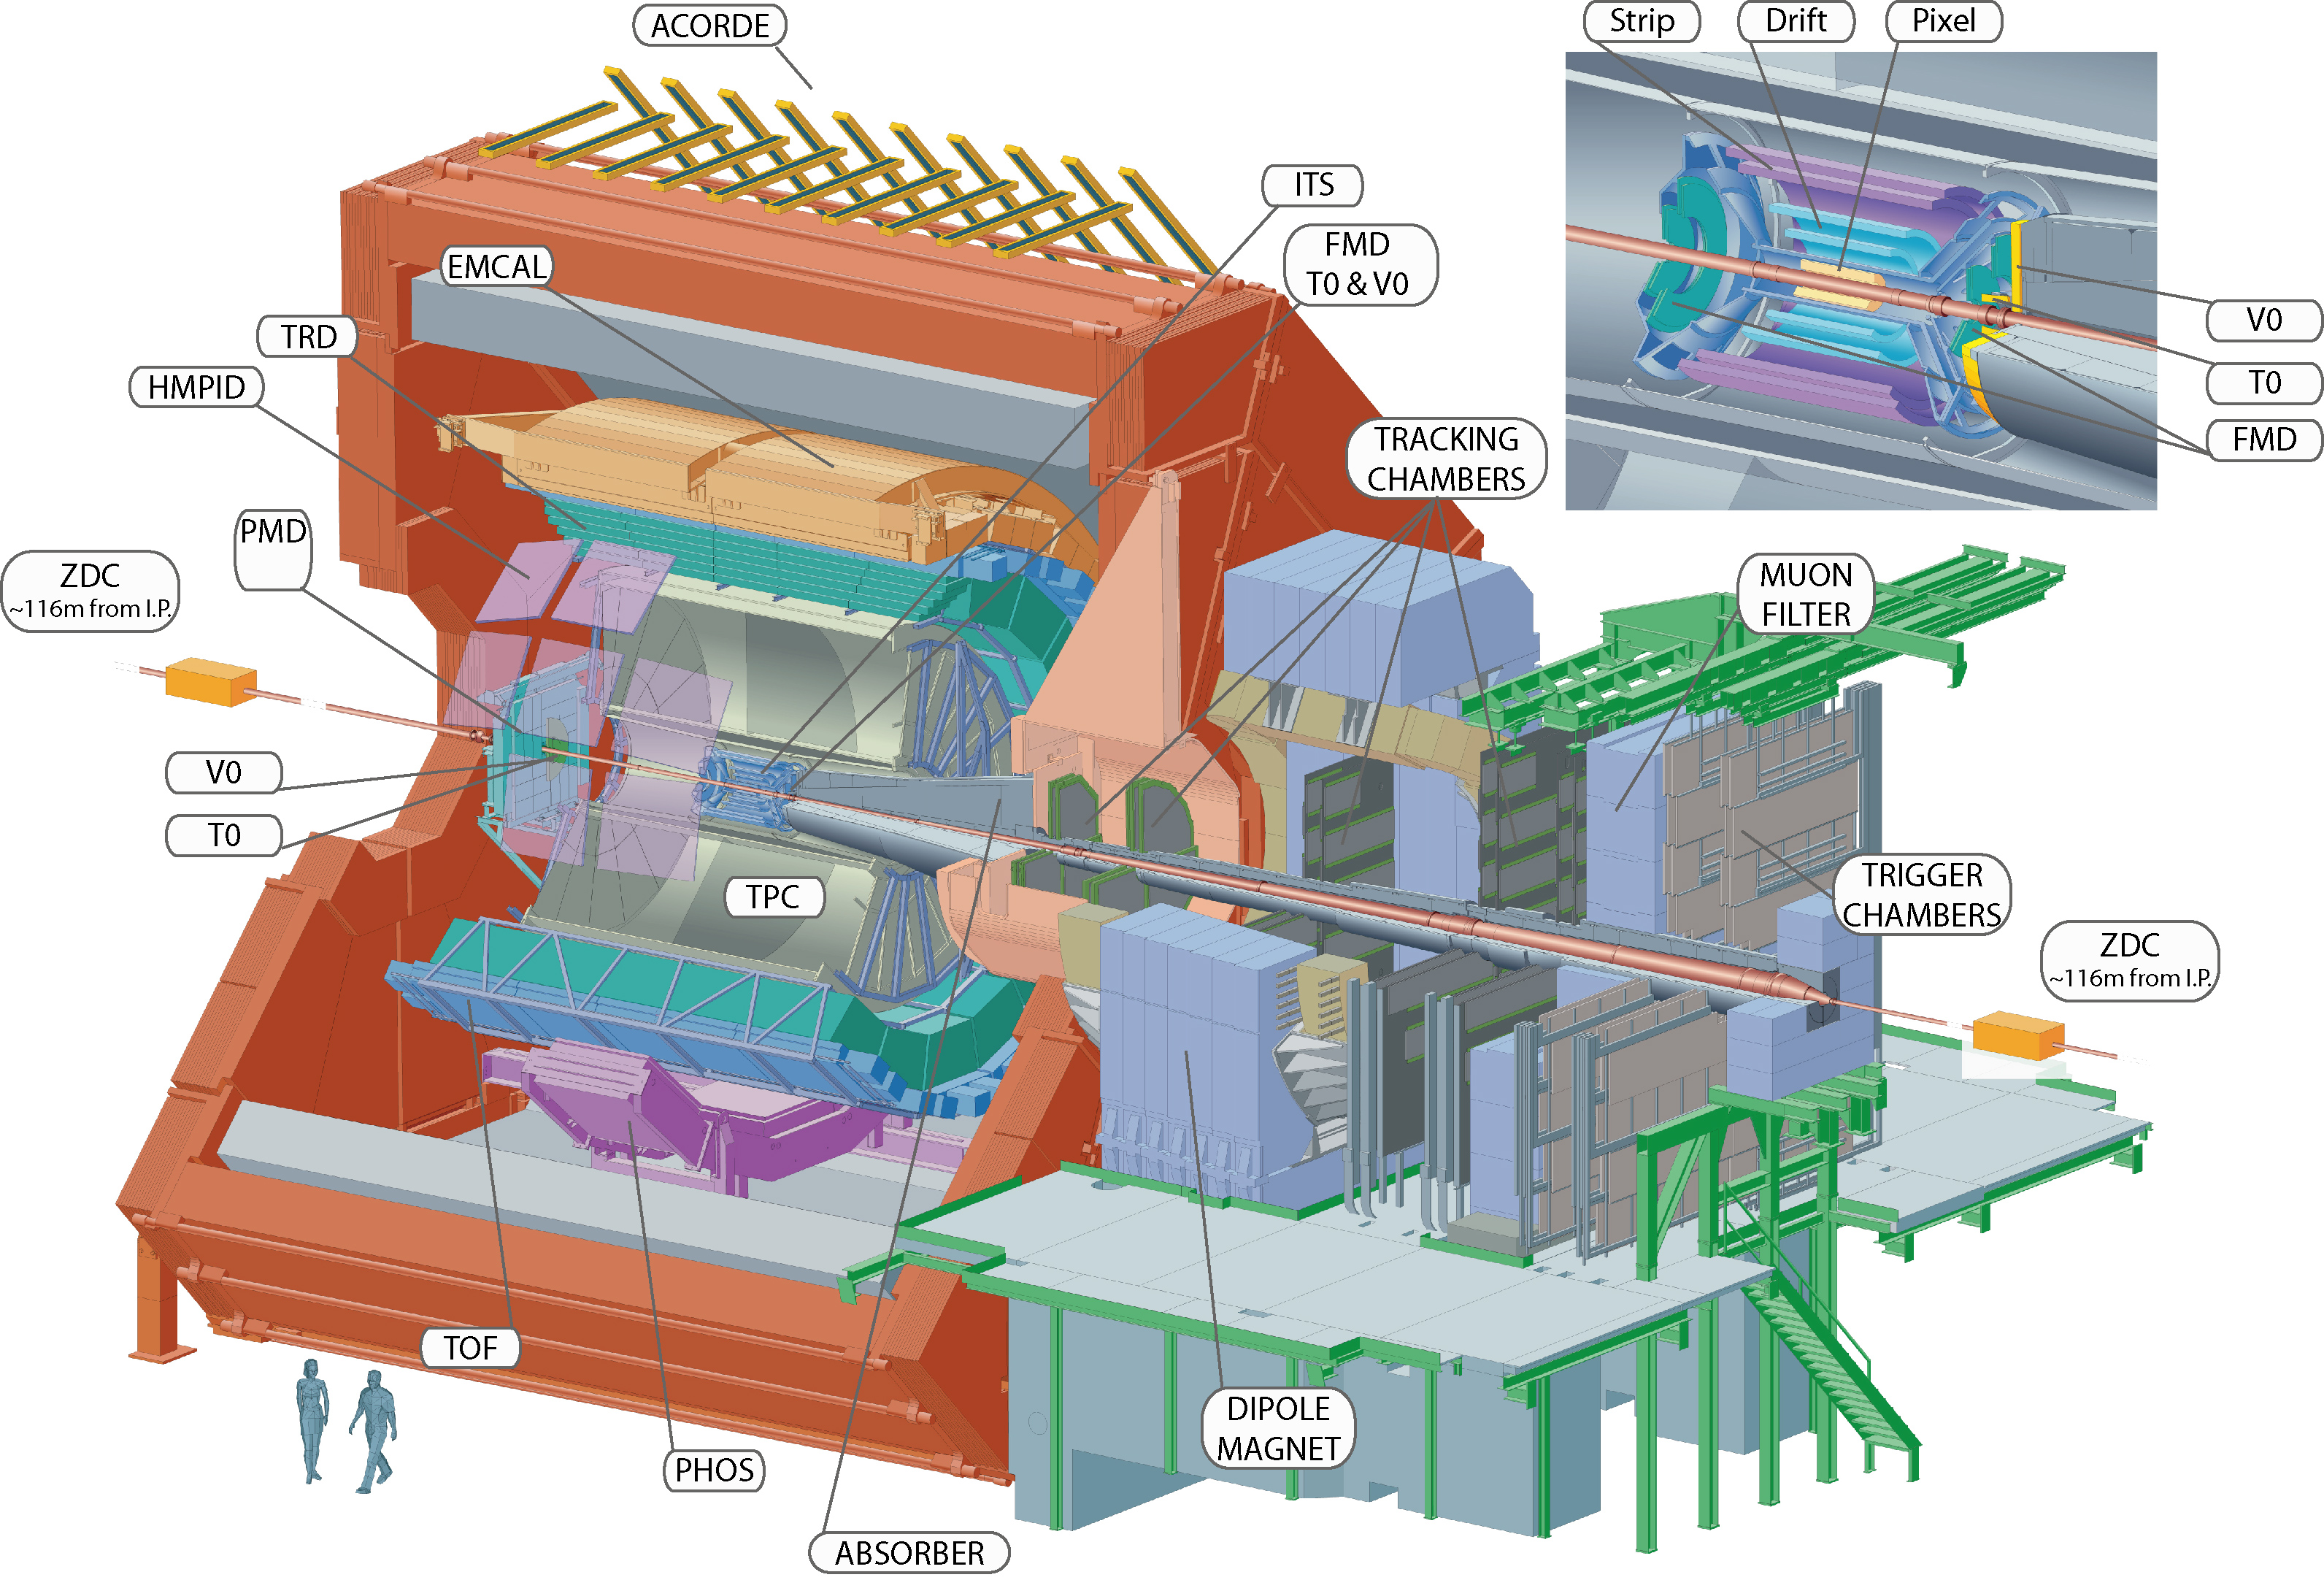
\includegraphics[width=\textwidth]{image/1-alice/alice.jpg}
    \captionwithsource{Schematica dei principali rilevatori presenti in ALICE. La struttura rossa che incapsula il \textit{central barrel} è l'\emph{L3 Magnet}.}{\href{https://en.wikipedia.org/wiki/ALICE_experiment\#/media/File:2012-Aug-02-ALICE_3D_v0_with_Text_(1)_2.jpg}{Wikimedia Commons}.}
    \label{fig:alice}
\end{figure}
Come già anticipato, nel \textit{central barrel} vi sono i rilevatori più importanti per la misura degli osservabili fisici.
Si elencano tramite una lista questi rilevatori, a partire da quello più interno a quello più esterno.

\subsubsection{L'\textit{Inner Tracking System} (ITS)}
L'\emph{Inner Tracking System}, con un diametro di appena 87 cm, ha il compito di localizzare i vertici primari delle collisioni, di ricostruire i vertici secondari, di identificazione di particelle con basso impulso trasverso ($p_t \sim 100$ MeV/$c$), tutto attraverso l'utilizzo di rilevatori al silicio, disposti in 6 piani concentrici.
L'ITS, essendo il rilevatore più interno, deve assicurarsi di raccogliere i dati con più precisione possibile perché è più vicino al luogo di interazione tra le particelle, quindi raccoglierebbe le particelle con minor vita media.
Per esempio i due stati più interni possiedono un potere risolutivo migliore di 100 \si{\micro\metre}.

\subsubsection{La \textit{Time Projection Chamber} (TPC)}
La \emph{Time Projection Chamber} è il principale rivelatore di tracciamento del \textit{central barrel}.
Essa presenta una simmetria assiale, con al centro un elettrodo ad alto voltaggio, e la superficie esterna che fa da gabbia di Faraday.
Con questa struttura le dimensioni del raggio interno ed esterno assumono il valore di $\sim 85$ cm e di $\sim 250$ cm rispettivamente.
Il compito principale della TPC è quello di misurare l'impulso di particelle cariche e di effettuare PID misurando l'energia persa per unità di distanza $dE/dx$, per particelle con $|\eta| < 0.9$.
Per la misura di questa grandezza, il volume interno è riempito con un gas (che durante \textit{Run} 2 consisteva in una miscela composta all'88\% da Ar e al 12\% da CO$_2$).
La particella perde energia per ionizzazione rilasciando  elettroni che quindi migreranno verso gli elettrodi, e il numero di elettroni rilevati sarà proporzionale alla perdita di energia della particella nel gas.

\subsubsection{Il rilevatore \textit{Time Of Flight} (TOF)}
Il rilevatore di tempo di volo \emph{Time-Of-Flight} consiste in una griglia cilindrica di rilevatori a piani resistivi multi-gap (MRPC), i quali misurano il tempo di volo delle particelle ottenendo in questo modo la loro velocità tramite la quale, insieme alla quantità di moto, è possibile ottenere la massa.
Il rilevatore ha una superficie di 141 \si{m^2} e riesce a misurare particelle con pseudo-rapidità centrale ($|\eta| < 0.9$).

\subsubsection{Il rilevatore \textit{High Momentum Particle IDentification} (HMPID)}
Il rilevatore di HMPID è dedicato all'identificazione di adroni carichi con $p_t > 1$ GeV/$c$, quindi serve come ausilio alla PID per gli altri rilevatori elencati in precedenza.
Tuttavia, questo strumento non riesce a rilevare particelle con $|\eta| >0.6$, limitando la statistica disponibile.

\subsubsection{Altri rilevatori}
Altri rilevatori sono:
\begin{itemize}
    \item Gli \emph{Zero Degree Calorimeter}, usati ad esempio per contare il numero di nucleoni spettatori, cioè che non partecipano alla collisione;
    \item Il \emph{V0 detector}, composto da due griglie circolari di scintillatori, ognuno posto sull'asse di collisione in punti opposti rispetto al punto di interazione, misurando in questo modo particelle con alta rapidità.
    Essi funzionano emettendo un segnale con intensità proporzionale al numero di particelle che li attraversano, dunque possono essere usati per la determinazione della molteplicità e della centralità a seconda della collisione considerata;
    \item Il \emph{T0 detector}, formato da due contatori Cherenkov, collocati nella stessa modalità in cui sono disposti i \textit{V0 detector}.
    Vista la disposizione spaziale, anch'essi si occupano di particelle con alta rapidità.
    Una delle loro funzioni è quella di fornire una misura precisa del tempo di collisione degli eventi, necessaria per le misure del tempo di volo.
    Esse possono essere anche utilizzate per la determinazione della posizione del vertice, tuttavia con minore precisione ($\pm 1.5$ cm).
\end{itemize}

L'identificazione di nuclei e antinuclei leggeri in ALICE viene effettuata attraverso la misura della perdita di energia specifica ($dE/dx$) e del tempo di volo delle tracce cariche effettuata da TPC e TOF, rispettivamente.
Ogni particella, infatti, assume un proprio andamento caratteristico della perdita di energia $dE/dx$ in funzione della quantità di moto.
A dimostrazione, la \autoref{fig:pid} mostra alcuni rari candidati di $^4\overline{\text{He}}$ identificati con successo nella presa dati del 2011 \cite{refId0_exotica}.
\begin{figure}[ht]
    \centering
    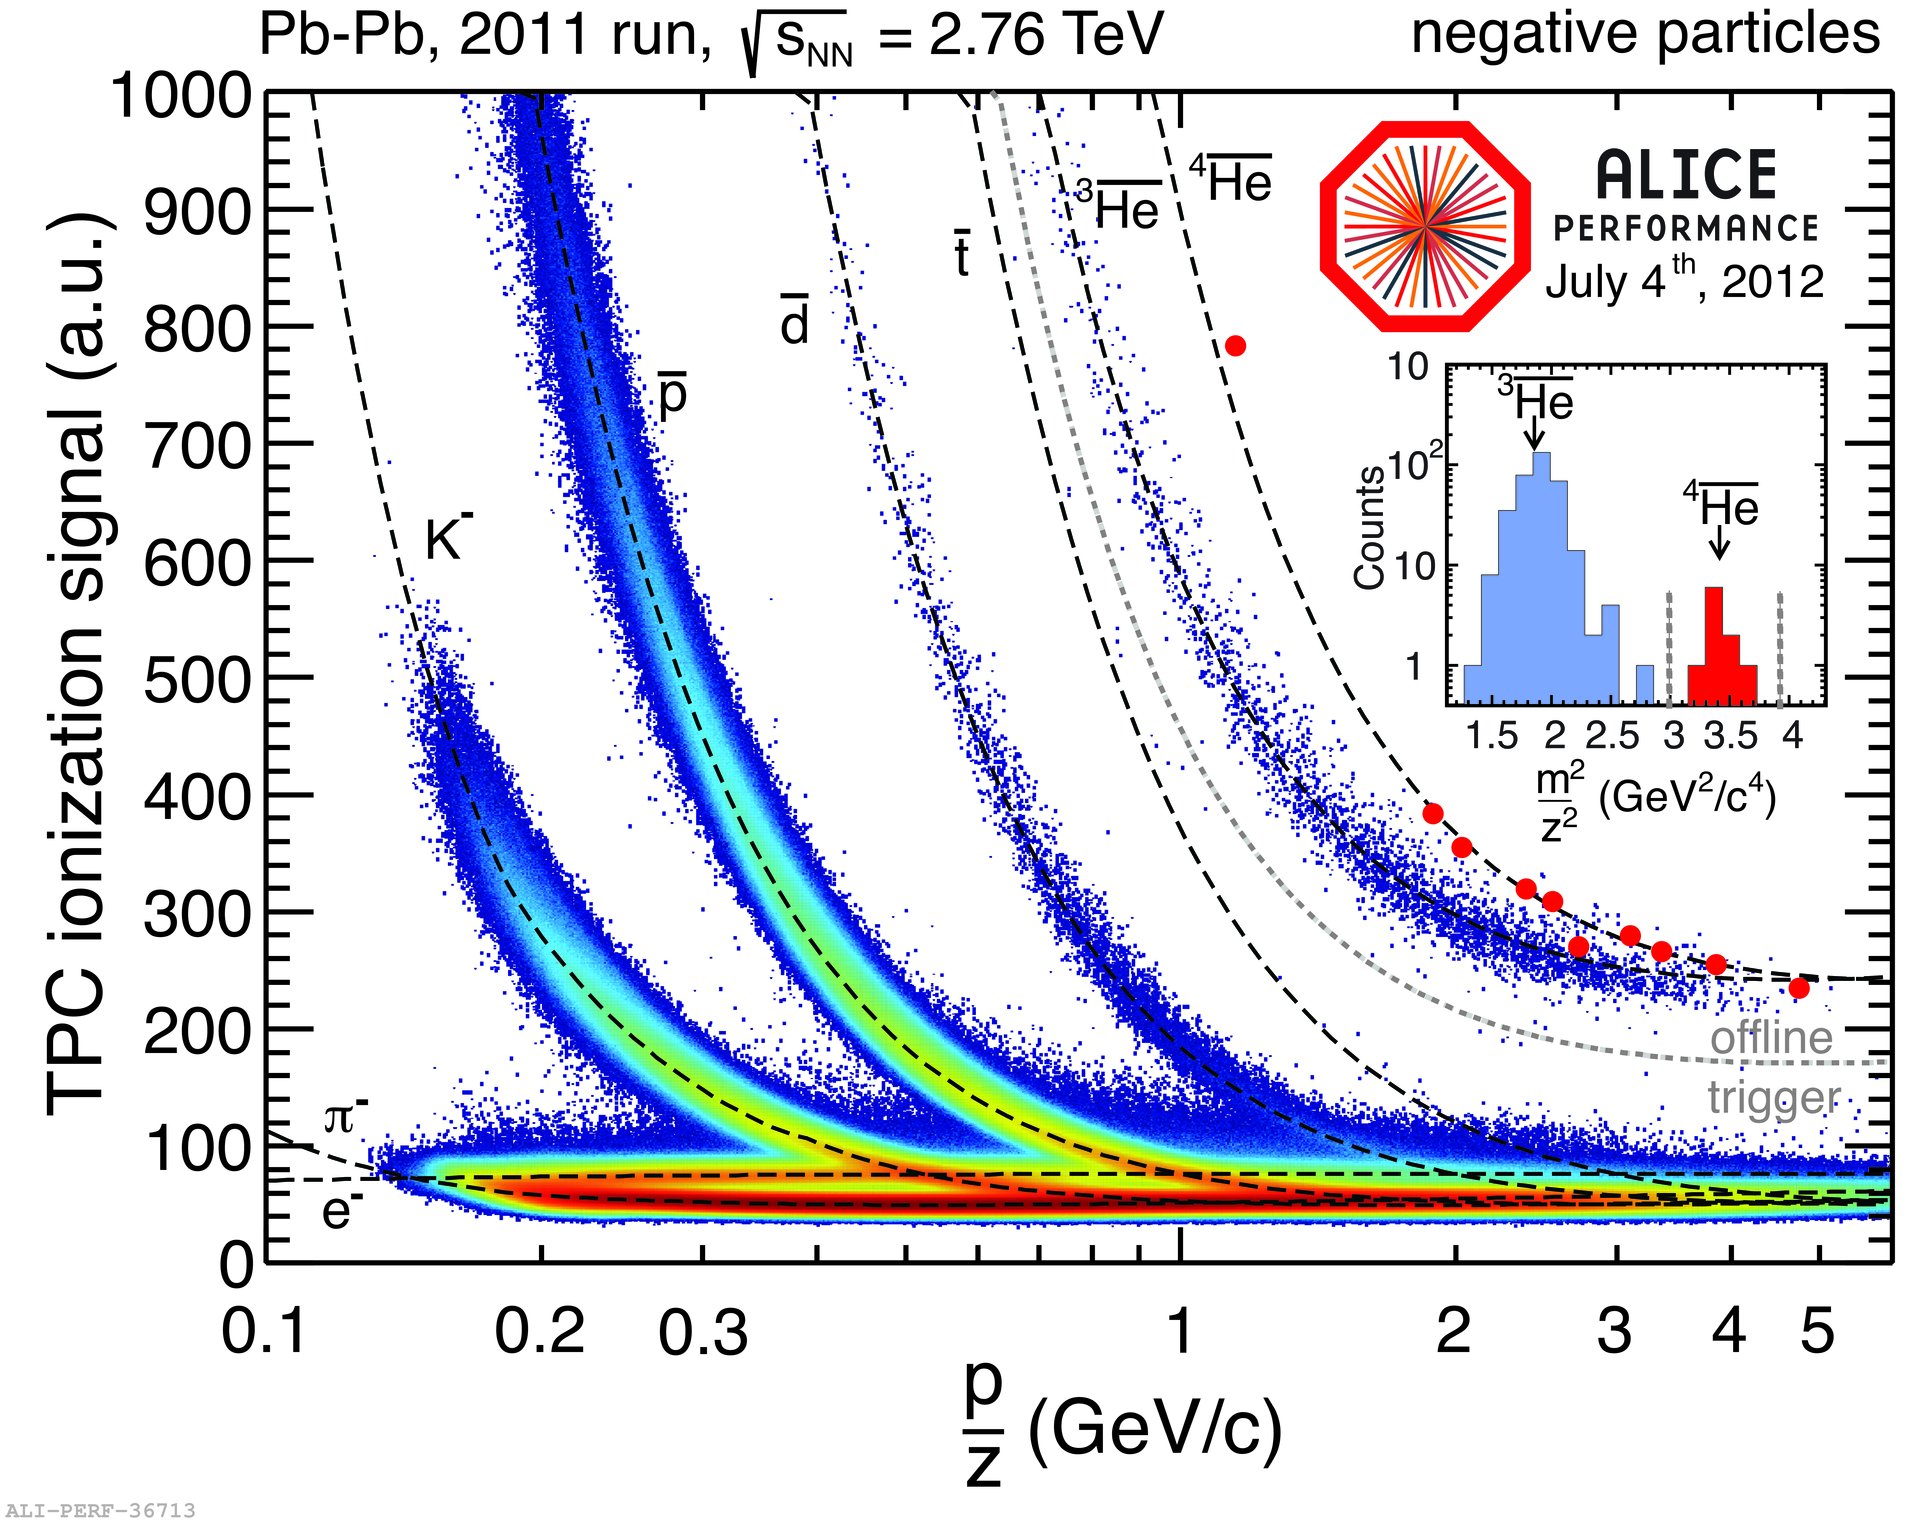
\includegraphics[width=0.7\linewidth]{image/1-alice/PID.png}
    \captionwithsource{Spettro misurato dalla TPC della perdita di energia specifica di particelle con carica negativa. Le linee tratteggiate rappresentano le previsioni teoriche, mentre i punti rossi rappresentano i candidati di $^4\overline{\text{He}}$ selezionati utilizzando la misura del tempo di volo delle anti-particelle. $\bar d$ rappresenta gli antideuteroni, $\bar t$ indica gli anti-trizi.}{\cite{refId0_exotica}}
    \label{fig:pid}
\end{figure}